% Figure: Worked example — C to CSimpl to L1 to proof
\begin{figure*}[t]
\centering
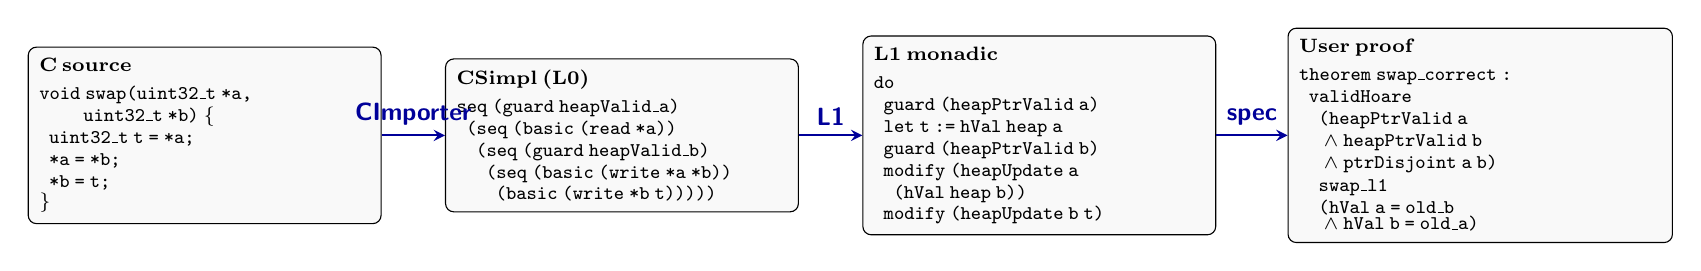
\begin{tikzpicture}[
  cbox/.style={draw, rounded corners=3pt, fill=gray!5,
               text width=4.2cm, font=\ttfamily\tiny, align=left,
               inner sep=4pt},
  arrow/.style={->, >=stealth, thick, color=blue!60!black},
  stagelabel/.style={font=\small\sffamily\bfseries, text=blue!60!black},
]
  % C source
  \node[cbox] (csrc) at (0, 0) {
    \normalfont\scriptsize\textbf{C source}\\[2pt]
    \texttt{void swap(uint32\_t *a,}\\
    \texttt{\ \ \ \ \ \ \ \ \ uint32\_t *b) \{}\\
    \texttt{\ \ uint32\_t t = *a;}\\
    \texttt{\ \ *a = *b;}\\
    \texttt{\ \ *b = t;}\\
    \texttt{\}}
  };

  % CSimpl
  \node[cbox] (csimpl) at (5.3, 0) {
    \normalfont\scriptsize\textbf{CSimpl (L0)}\\[2pt]
    \texttt{seq (guard heapValid\_a)}\\
    \texttt{\ \ (seq (basic (read *a))}\\
    \texttt{\ \ \ \ (seq (guard heapValid\_b)}\\
    \texttt{\ \ \ \ \ \ (seq (basic (write *a *b))}\\
    \texttt{\ \ \ \ \ \ \ \ (basic (write *b t)))))}
  };

  % L1 monadic
  \node[cbox] (l1) at (10.6, 0) {
    \normalfont\scriptsize\textbf{L1 monadic}\\[2pt]
    \texttt{do}\\
    \texttt{\ \ guard (heapPtrValid a)}\\
    \texttt{\ \ let t := hVal heap a}\\
    \texttt{\ \ guard (heapPtrValid b)}\\
    \texttt{\ \ modify (heapUpdate a}\\
    \texttt{\ \ \ \ (hVal heap b))}\\
    \texttt{\ \ modify (heapUpdate b t)}
  };

  % Proof
  \node[cbox, text width=4.6cm] (prf) at (16.2, 0) {
    \normalfont\scriptsize\textbf{User proof}\\[2pt]
    \texttt{theorem swap\_correct :}\\
    \texttt{\ \ validHoare}\\
    \texttt{\ \ \ \ (heapPtrValid a}\\
    \texttt{\ \ \ \ \ $\wedge$ heapPtrValid b}\\
    \texttt{\ \ \ \ \ $\wedge$ ptrDisjoint a b)}\\
    \texttt{\ \ \ \ swap\_l1}\\
    \texttt{\ \ \ \ (hVal a = old\_b}\\
    \texttt{\ \ \ \ \ $\wedge$ hVal b = old\_a)}
  };

  % Arrows
  \draw[arrow] (csrc.east) -- node[above, stagelabel] {CImporter} (csimpl.west);
  \draw[arrow] (csimpl.east) -- node[above, stagelabel] {L1} (l1.west);
  \draw[arrow] (l1.east) -- node[above, stagelabel] {spec} (prf.west);

\end{tikzpicture}
\caption{Worked example: \texttt{swap} through the pipeline. C source is
parsed into CSimpl (deep embedding), lifted to L1 monadic form, then
proven correct using Hoare logic with heap disjointness.}
\label{fig:worked}
\end{figure*}
